% Version 2006-12-05
\documentclass[12pt]{dalcsthesis}

%Figures -- these packages let you do some extra things with figures.
\usepackage[dvips]{graphicx}
\usepackage{subfigure}

\begin{document}

\mcs  % options are \mcs, \macs, \mec, \mhi, \phd, and \bcshon
\title{The title}
\author{Noah Body}
\defenceday{1}
\defencemonth{November}
\defenceyear{2006}
\convocation{May}{2007}

% Use multiple \supervisor commands for co-supervisors.
% Use one \reader command for each reader.

\supervisor{D. Prof}
\reader{D. Odaprof}
\reader{A. External}

\nolistoftables
\nolistoffigures

\frontmatter

\begin{abstract}
This is a test document.
\end{abstract}

\begin{acknowledgements}
Thanks to all the little people who make me look tall.
\end{acknowledgements}

\mainmatter

\chapter{Introduction}

Get it done!  Use reference material by Lamport~\cite{latex-by-lamport} or
Gooses, Mittelback, and Samarin~\cite{latex-companion}.

\chapter{Doing It}

\section{Getting Ready}

Get all the parts that I need.  I can throw in a whole pile of terms like
preparation,
methodology,
forethought,
and
analysis
as examples for me to use in the future.

\section{Next Step}

Do it!

Of course, you have to have pictures to show how you did it to make people
understand things better.

Every dissertation should consider having nice figures like Figure~\ref{fig-steiner_growth}.

\begin{figure}
  \centering
     {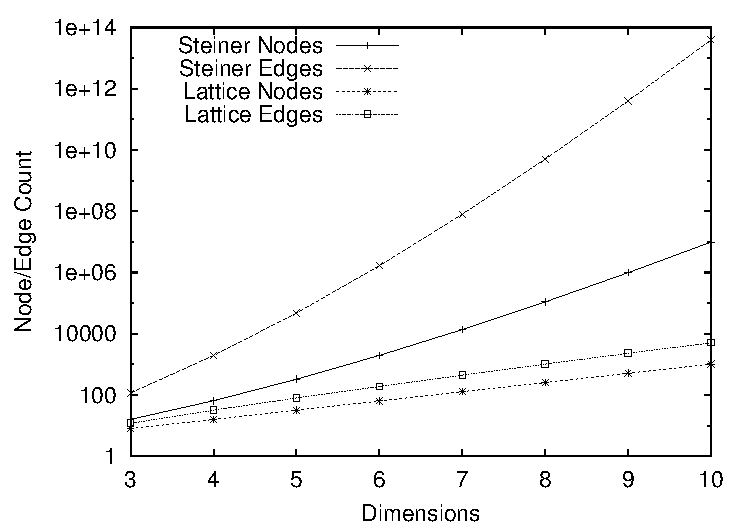
\includegraphics[height = 3.0 in]{samplefig}}
  \caption{\label{fig-steiner_growth} Growth patterns for Steiner
    graph versus original lattice. Note the logarithmic scale.}
\end{figure}

Sometimes it is useful to group figures together. 
Figure~\ref{fig-partial_compare} is an example of using the subfigure style.

\begin{figure}
  \centering
  \subfigure[Caption A]{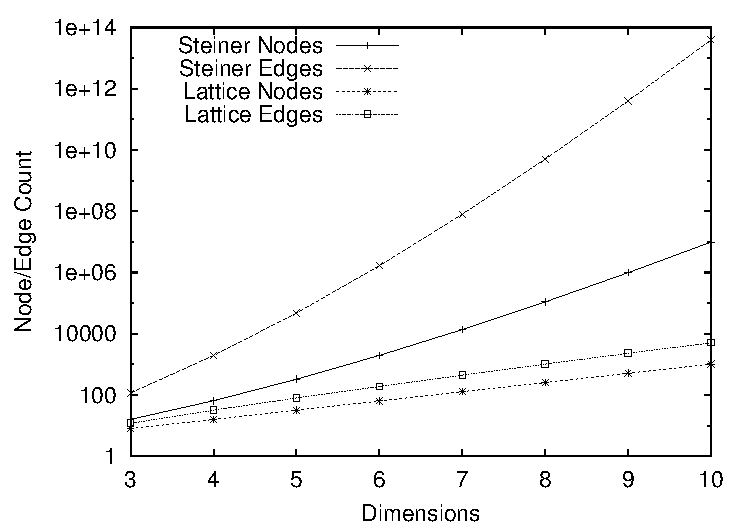
\includegraphics[width = 2.75 in]{samplefig}}\qquad
  \subfigure[Caption B]{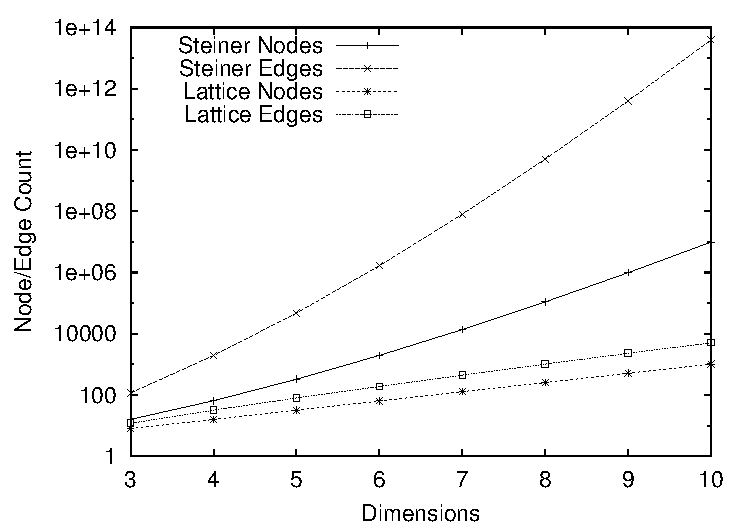
\includegraphics[width = 2.75 in]{samplefig}}\qquad
  \subfigure[Caption C]{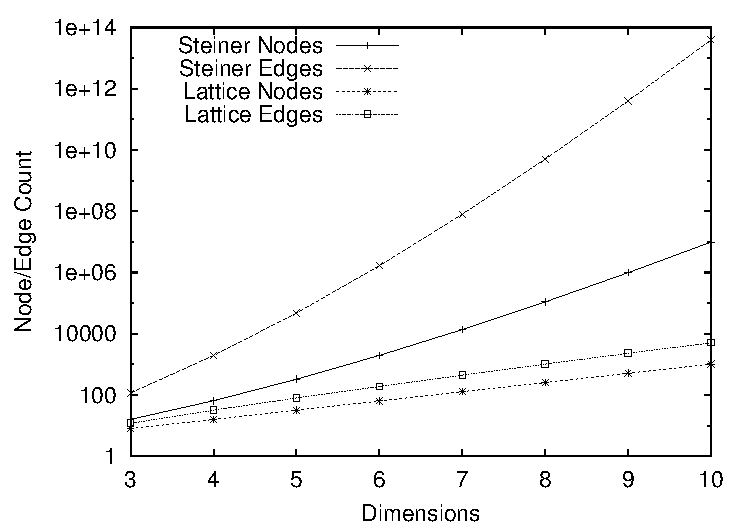
\includegraphics[width = 2.75 in]{samplefig}}\qquad
  \subfigure[Caption D]{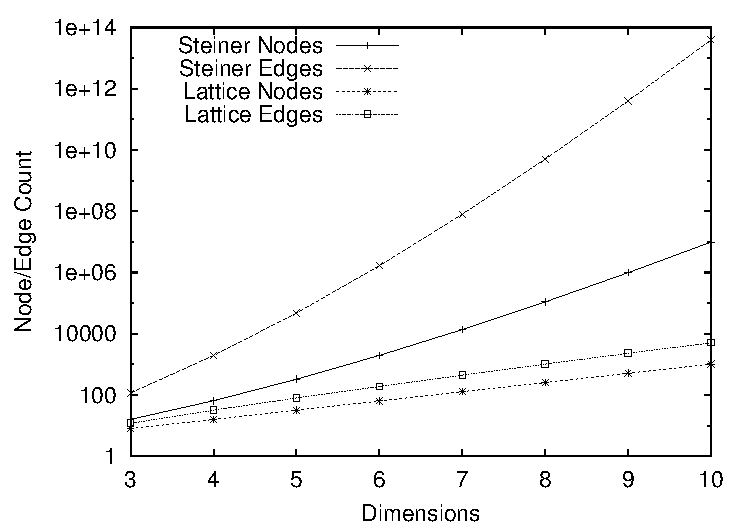
\includegraphics[width = 2.75 in]{samplefig}}
  \caption{\label{fig-partial_compare}Relative weight reduction for the
  schedule trees produced on subsets of size (a) 10\% (b) 25\% (c)
  50\% (d) 75\%. The baseline in this case is chosen as the
  smaller of (i) a sort of the raw data set for each view or (ii)
  computation of the full cube.}
\end{figure}

Thanks to Todd Eavis for providing the figures and usage method for the package.

\chapter{Conclusion}

Did it!

\bibliographystyle{plain}
\bibliography{simple}

\end{document}
